\documentclass{iopconfser}

\usepackage{graphicx}
\usepackage{amsmath,amssymb}
\usepackage[separate-uncertainty=true]{siunitx}
\usepackage{booktabs}
\usepackage{cite}
\usepackage{hyperref}
\usepackage{placeins}
\usepackage{wrapfig}
\graphicspath{{figures/}}
\renewcommand{\topfraction}{0.9}
\renewcommand{\bottomfraction}{0.8}
\renewcommand{\textfraction}{0.1}
\renewcommand{\floatpagefraction}{0.85}

\begin{document}

\title{Gamma detection for source localisation in targeted alpha therapy}

\author{C. De Sio$^{1}$, L. Abu Sabah$^{1}$, J. Duan$^{1}$, Y. Shi$^{1}$,
S. Williams$^{1}$ and J. Velthuis$^{1}$}

\affil{$^1$School of Physics, University of Bristol, Bristol, United Kingdom}

\begin{abstract}
Targeted alpha therapies can deliver a highly localised dose to tumours, but treatment
planning and effectiveness depend on whether the radionuclide source remains near
the intended site after administration. In the AlphaGlue delivery concept,
alpha emitters are applied to a tumour region in a thin glue layer. We present
a Geant4 simulation study showing that decay-chain gamma detection can
distinguish retained, broadly diffused and locally displaced source states in
an AlphaGlue-like geometry. For each of the seven source configurations, 50
independent simulations of 10,000 primary events were generated, and
baseline-subtracted gamma-hit profiles were successfully used to reconstruct the broad diffusion
fraction with $R^2=0.9987$ and a mean absolute error of about one percentage
point. Displaced source activity was detected by gamma signal analysis and source position was reconstructed with mean
position errors of 16--30 mm. These results support gamma detection as a
candidate method for emitter-position monitoring, treatment planning and
delivery verification.
\end{abstract}

\section{Introduction}

\begin{wrapfigure}{r}{0.36\textwidth}
\centering
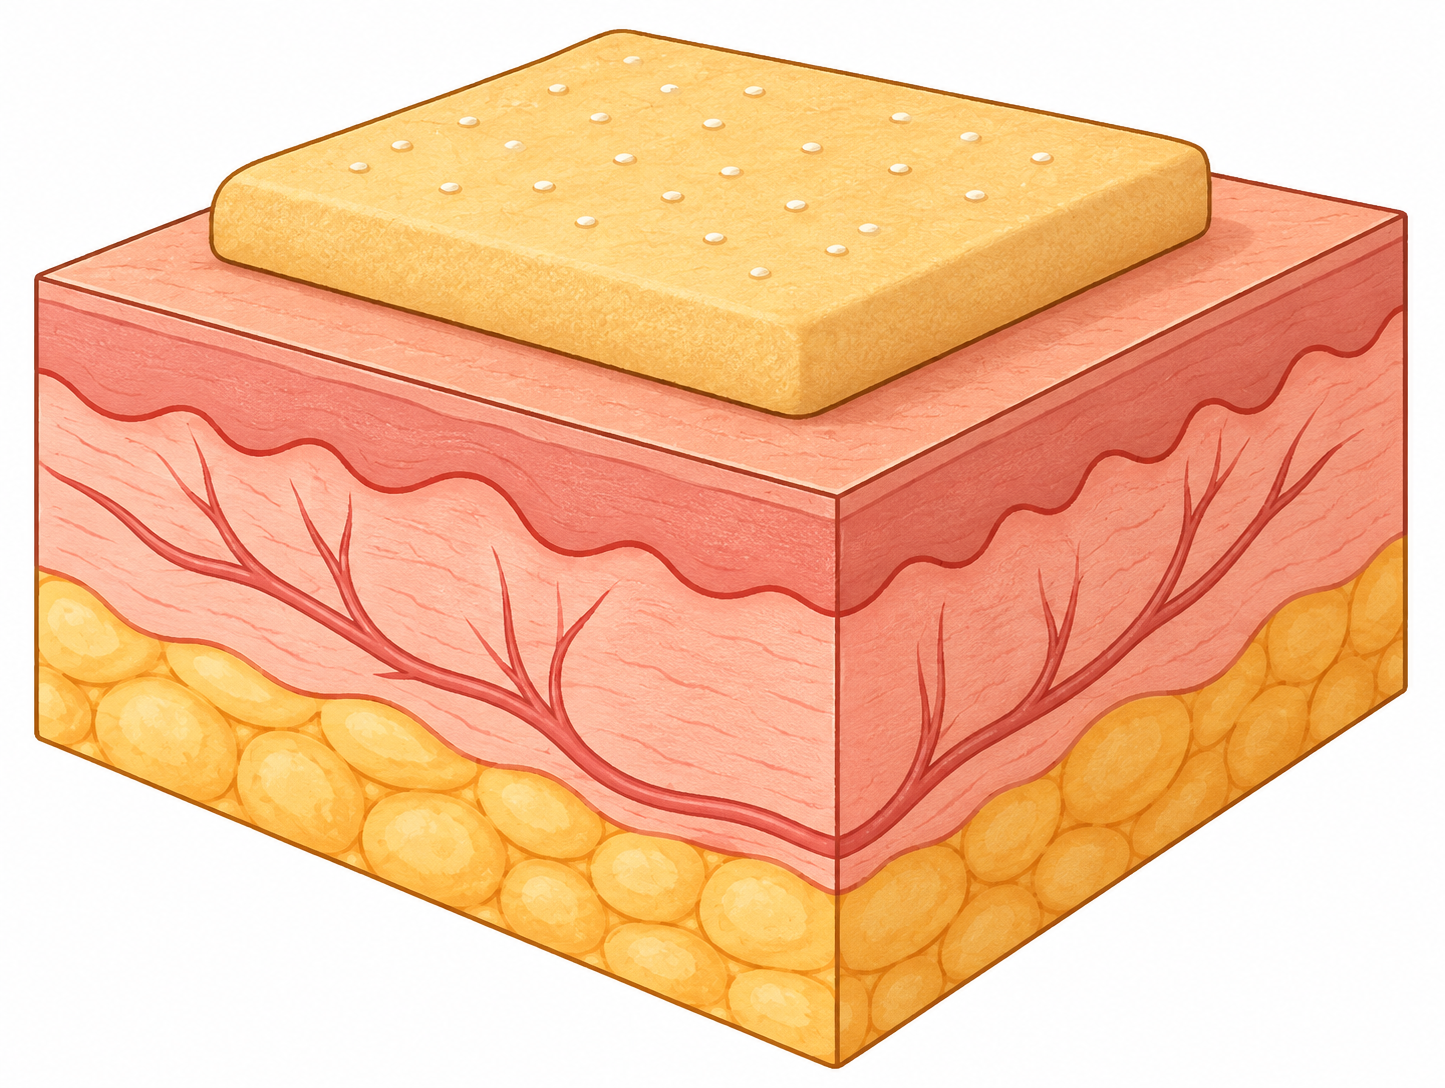
\includegraphics[width=\linewidth]{figures/AlphaGlue_Sketch.png}
\caption{Conceptual illustration of an AlphaGlue applicator placed on tissue.}
\label{fig:alphaglue_concept}
\end{wrapfigure}

In targeted alpha therapy, the delivered dose is strongly local. A treatment
plan therefore depends on the initial activity distribution and its evolution
after administration. The
\href{https://doi.org/10.3390/biomedinformatics5040058}{AlphaGlue concept}
proposes suspending alpha emitters in a thin glue layer applied to tissue
\cite{AlphaGlue2025}, as illustrated in Fig.~\ref{fig:alphaglue_concept}. The concept has previously been evaluated with Geant4
and Geant4-DNA simulations for dose and DNA-damage modelling
\cite{Geant4,Geant4DNA,CellCycleAlpha,At211,DartDoseDNA,DartInsilico}. Its
delivered dose depends on whether source material and progeny remain near the
intended deposition site, diffuse into surrounding tissue or are redistributed
by biological transport~\cite{laura,heger}. This study investigates whether the accompanying
gamma signal can be used as a theranostic observable to monitor emitter
position, detect source movement and provide useful information as a function
of detection time.

\section{Simulation model}

Photon transport was simulated with the Geant4 toolkit~\cite{Geant4}. The
model places a \(\SI{40}{mm} \times \SI{2}{mm} \times \SI{40}{mm}\) loaded
glue layer on the \(+y\) surface of a
\(\SI{20}{cm} \times \SI{20}{cm} \times \SI{150}{cm}\) water phantom. Six
detector panels surround the phantom at \(\SI{20}{cm}\) from the water
surface. Each photon entry into a detector panel is counted as one hit.

Radionuclides or their progeny may leave the applicator region by diffusing into surrounding tissue or entering the circulation and being transported by blood flow. This migration can produce a broad redistribution through the surrounding tissue, with large
variation reported between experiments~\cite{laura,heger}. To test whether these behaviours can be distinguished from source retention, seven source configurations were simulated. The retained-source configuration was used as the baseline. Broad redistribution was represented by cases in which 10\%, 50\% or 90\% of the source was distributed throughout the water volume. The localised-displacement scenario was represented by placing 20\%, 40\% or 60\% of the source in a \(\SI{5}{cm}\)-side water cube centred at
\((x,y,z)=(0,0,\SI{500}{mm})\), spanning \(475\leq z\leq525\) mm.

The geometry is described in Fig.~\ref{fig:geometry}, along with example detector displays showing the three clinical scenarios.
Each configuration was simulated with 50 independent repetitions of 10,000
primary decays, giving 500,000 simulated decays per configuration and
3.5 million simulated decays across all source states. The repeated runs
define the run-to-run uncertainty used in the residual and detectability
analysis. The simulated decays
are rescaled to a DaRT-like reference activity of
\(3~\mu\mathrm{Ci}\) (\(\SI{111}{\kilo\becquerel}\)), matching the order
of a single DaRT seed~\cite{dart}.

\begin{figure}[htbp]
\centering
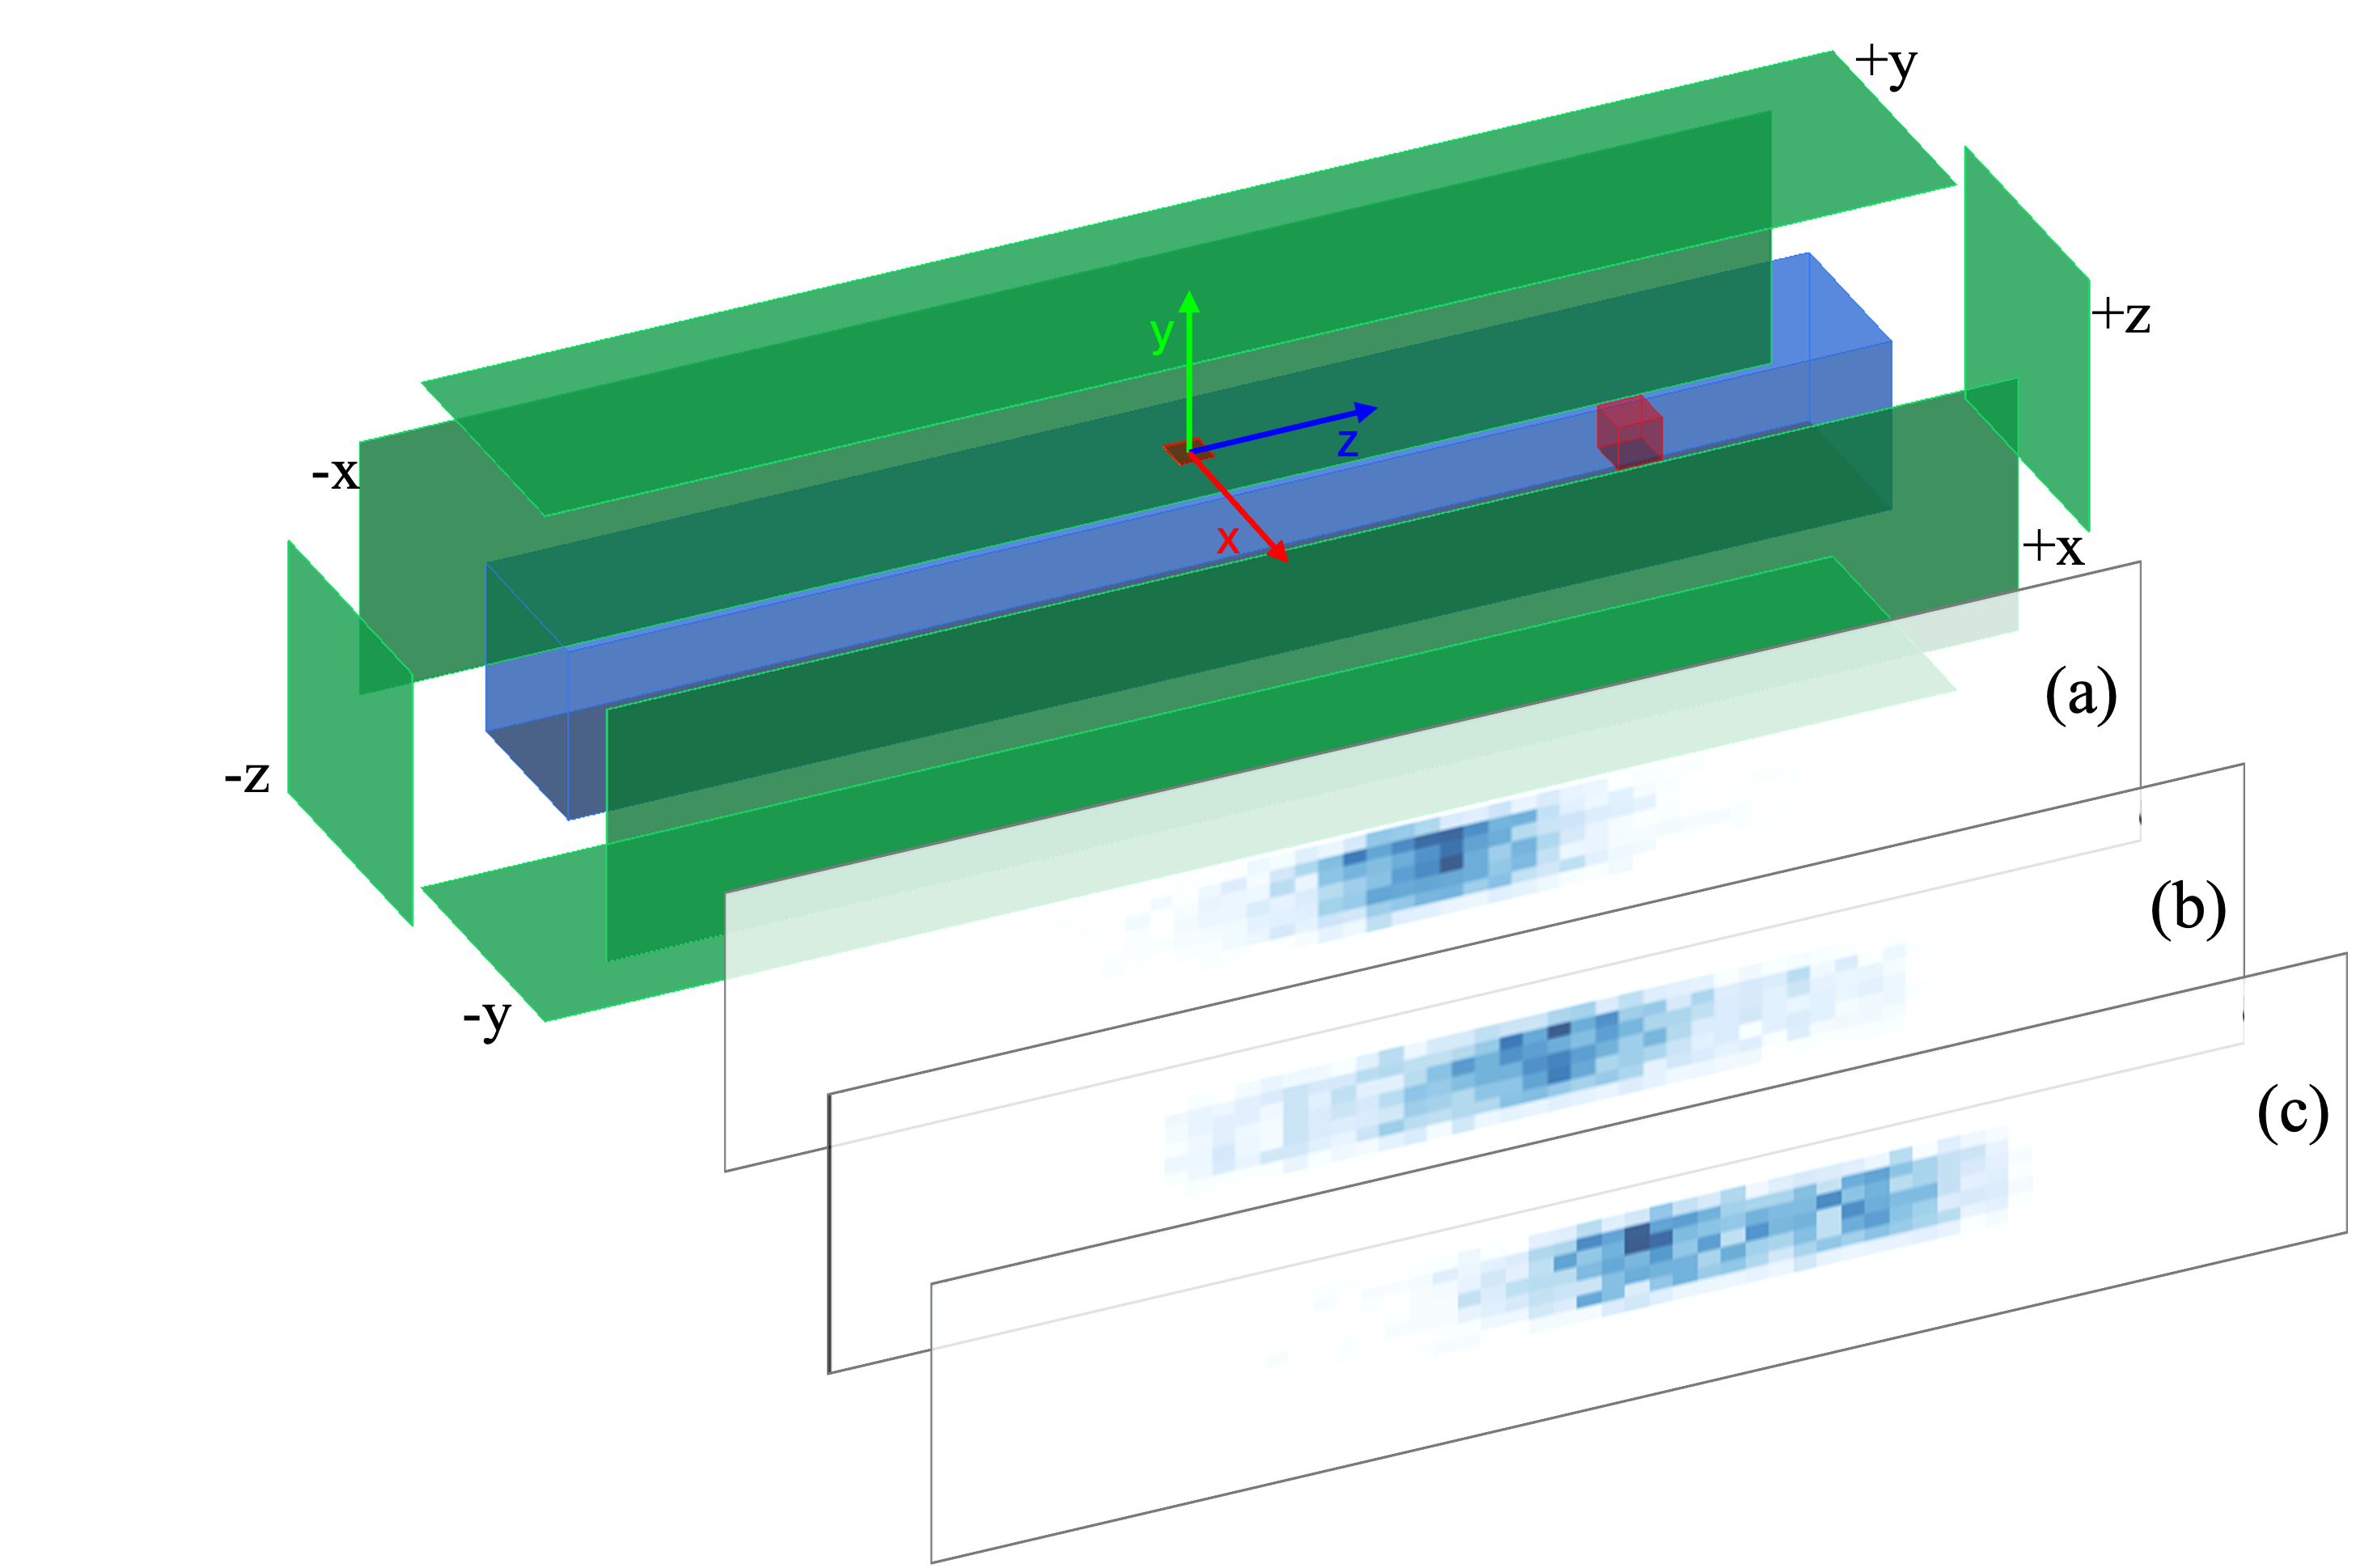
\includegraphics[width=0.72\linewidth]{figures/aocmp_paper_geometry_labels2.png}
\caption{Simulation geometry showing the water phantom (blue), AlphaGlue applicator region (red, centre), surrounding
detector panels (green), a displaced source (red, right side) and three offset example \(x\)-panel projections: baseline (a), broad redistribution (b), and displaced localisation (c).}
\label{fig:geometry}
\end{figure}

\section{Baseline subtraction}

Each photon entry into a detector panel was recorded as one hit, together with its detector panel and entry position. Detector panels are named according to the side of the phantom on which they are located. The \(+x\) and \(-x\) panels are the two lateral panels at positive and negative \(x\); the \(+y\) panel faces the AlphaGlue applicator and the \(-y\) panel lies on the opposite side. The \(+z\) and \(-z\) panels close the longitudinal ends of the geometry. These end panels recorded substantially fewer entries than the four side panels and were not included in the present quantitative analysis. A combined \(x\)-panel profile is obtained by summing the \(+x\)- and \(-x\)-panel counts bin by bin and plotting them against the longitudinal coordinate \(z\). Thus, ``\(x\)-panel'' identifies the detector location, while \(z\) identifies position along the panel. Longitudinal profiles were examined because redistribution changes the spatial pattern of detector hits more strongly than the total number of hits. The total detector-entry rate differed by only 3.8\% between the retained baseline and the 90\% broad-diffusion case, whereas subtraction of the retained-source profile revealed clear spatial differences (Fig.~\ref{fig:residual_profiles}). The retained
source defines the reference profile \(\bar{h}^{B}_{p}(z)\) for detector panel
\(p\). Candidate source states are represented by
\begin{equation}
\Delta h_p(z)=h_p(z)-\bar{h}^{B}_{p}(z),
\end{equation}
with the repeated baseline simulations defining the bin-wise noise scale. Each profile was divided by the number of simulated primary decays and rescaled to the initial emitter population corresponding to the \(3~\mu\mathrm{Ci}\) reference activity. The plotted residual is the difference between the mean activity-scaled candidate and retained-source profiles. Positive residuals mark detector
regions where the candidate produces more gamma entries than the
retained-source case, while negative residuals mark depleted regions. In the
combined (x)-panel projection, broad diffusion widens the residual pattern,
whereas localised displacement produces a shifted excess near the displaced
source region. Changes in the balance between the glue-facing and opposite
detector panels provide an additional feature for the quantitative analysis.

\begin{figure}[htpb]
\centering
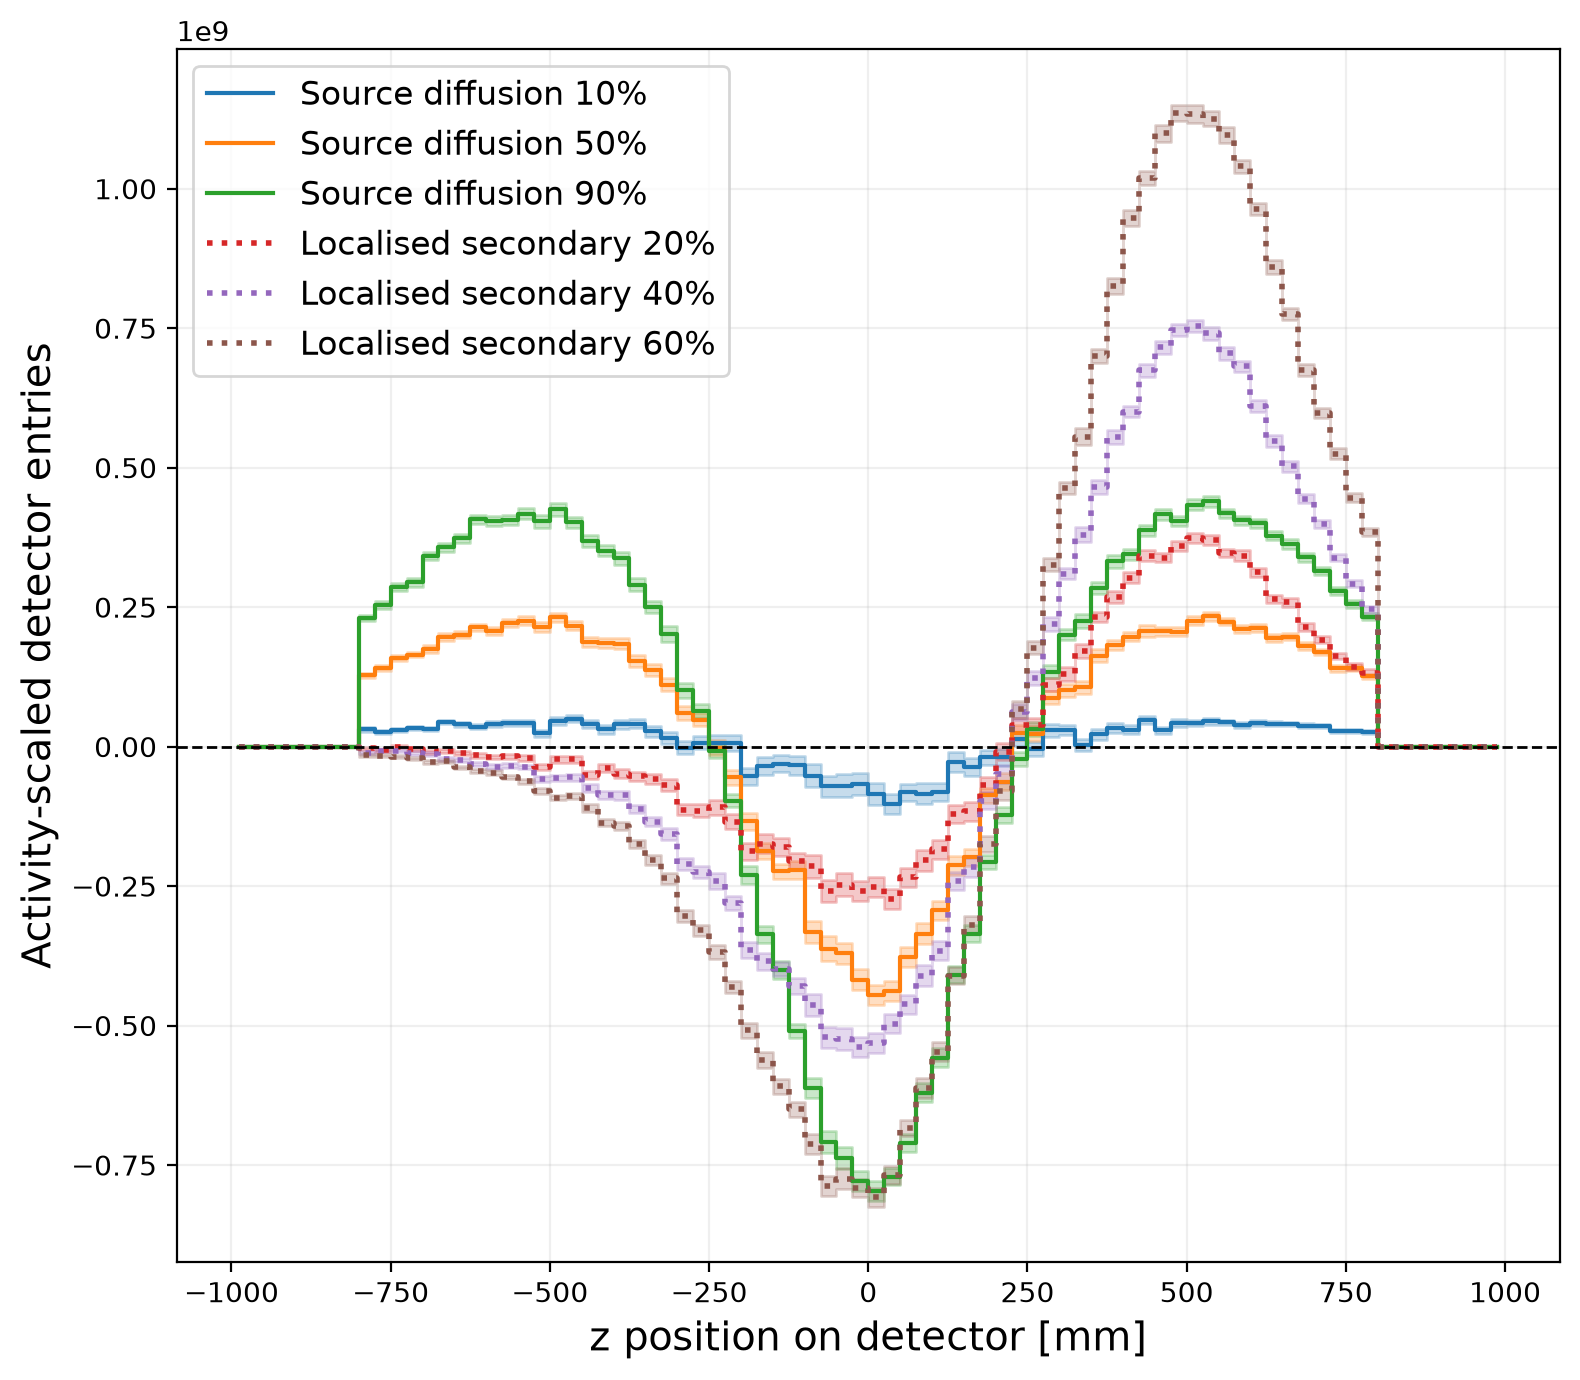
\includegraphics[width=0.65\linewidth]{poster_01_baseline_subtracted_profiles_xsum_all_cases.png}
\caption{Activity-scaled, baseline-subtracted combined \(+x\) and \(-x\) detector
profiles for broad diffusion and localised displacement. Shaded bands show the
propagated standard error of the mean across 50 repetitions.}
\label{fig:residual_profiles}
\end{figure}

As an illustration of the general ROI strategy, Fig.~\ref{fig:leakage_roi}
compares the full longitudinal profile formed by summing the \(+x\) and \(-x\) panel counts with a region at \(-750\leq z\leq-550\) mm, where little signal is
expected from retained activity. An excess in this region indicates that the
detected distribution has spread beyond the applicator footprint. This ROI
illustrates the principle on which the quantitative estimators in
Section~\ref{sec:signal_analysis} are based: source redistribution is inferred
from spatial changes relative to the retained-source reference.

\begin{figure}[htbp]
\centering
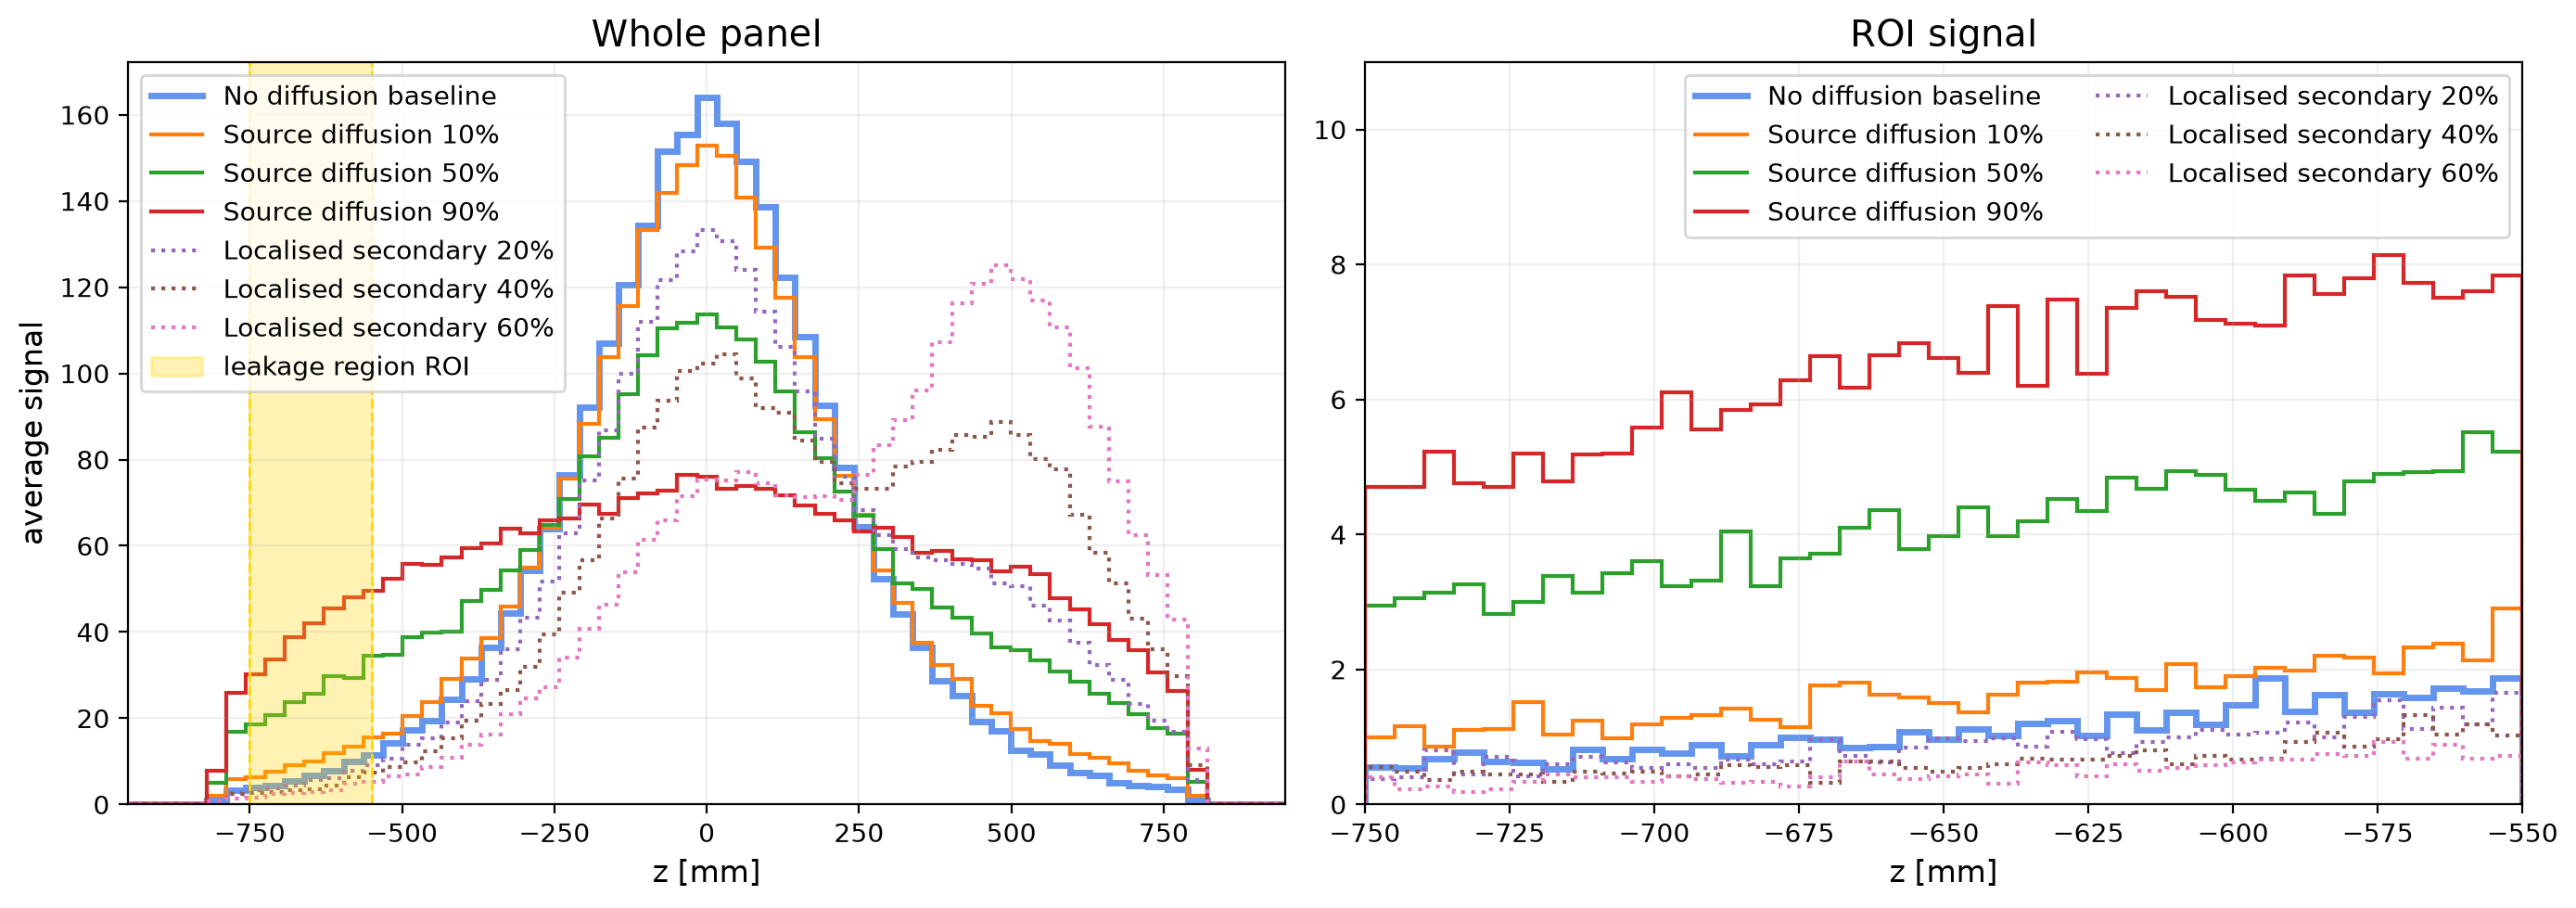
\includegraphics[width=0.98\linewidth]{poster_03c_leakage_roi_side_by_side.png}
\caption{Combined \(+x\)/\(-x\) longitudinal profiles (left) and an illustrative low-signal ROI
(right). The ROI highlights the broad-diffusion excess outside the
retained-source region.}
\label{fig:leakage_roi}
\end{figure}

\section{Signal analysis and source redistribution metrics}
\label{sec:signal_analysis}

The signal analysis addresses four tasks: detecting and locating a compact secondary
source, estimating the broadly diffused fraction when no compact source is
present, estimating how much signal remains consistent with the applicator
region, and determining the observation time required to distinguish each
candidate from the retained-source baseline. Together, these tasks determine whether activity has moved, whether the redistribution is broad or localised, where a compact displaced source is located, and how quickly each change becomes detectable. Both broad diffusion and compact
displacement can reduce the central signal, so the compact-secondary test is
applied first. A negative result enables the broad-diffusion and
applicator-retention estimates; a positive result instead triggers source
localisation.

\subsection{Compact secondary-source detection and localisation}

Counts and spatial-profile features from the four side panels were used to distinguish a compact displaced source from retained and broadly redistributed source states. The panel asymmetries were calculated as
\[
A_i=\frac{N_{+i}-N_{-i}}{N_{+i}+N_{-i}},\qquad i\in\{x,y\},
\]where \(N_{+i}\) and \(N_{-i}\) are the total numbers of entries on the opposing side panels. Broad diffusion primarily changes \(A_y\), because activity moves away from the applicator-facing \(+y\) panel, while a source displaced along \(z\) produces a shifted feature within the longitudinal detector profiles.
Compact-source detection used a balanced logistic-regression classifier supplied with standardised panel asymmetries, baseline-subtracted profile bins, positive-residual integrals, peak and centroid positions, longitudinal widths, ROI rates and the total detected rate. Performance was evaluated using leave-one-repetition-out validation.

A displaced-source ROI of \(250\leq z\leq750\) mm was defined in the combined \(+x/-x\) and \(+y/-y\) longitudinal profiles. For each view, the ROI signal was obtained by summing the positive candidate-minus-baseline residual over all \(z\) bins in this interval. After positive detection, the source position was estimated from the positive-residual centroid separately in the combined \(x\)- and \(y\)-panel profiles. The final position estimate was the mean of these two centroids.
\[
\hat z_{\mathrm{sec}}=
\frac{\hat z_{X\mathrm{sum}}+\hat z_{Y\mathrm{sum}}}{2},
\]
The reconstructed positions and their repetition-level residuals are reported
in Fig.~\ref{fig:source_residuals}.

\subsection{Broad-diffusion fraction}

Broad diffusion is estimated only after the compact-secondary test is
negative. Inputs comprise shape-normalised \(z\)-profile bins from the
combined \(x\), combined \(y\) and combined four-side-panel views; the standard deviation and central-$80\%$ interquantile width ($z_{90}-z_{10}$); the central \(+y\) fraction; \(x\)- and \(y\)-panel
asymmetries; absolute-residual integrals; and positive-residual centroid and peak-position summaries. These
features are standardised and supplied to ridge regression~\cite{RidgeRegression}. The ridge regularisation parameter, \(\alpha\), was selected by cross-validation from candidate values between \(10^{-4}\) and \(10^4\), balancing agreement with the training data against model complexity. The model is trained only on the retained and
10\%, 50\% and 90\% broad-diffusion states; localised-source cases are
excluded. Performance is evaluated with leave-one-repetition-out validation.
The resulting predictions are shown in Fig.~\ref{fig:diffusion_prediction}.

\subsection{Applicator-retained signal}

The applicator-facing observable is the \(+y\)-panel count in the central
ROI, \(|z|\leq150\) mm, normalised per primary event. Dividing this rate by
the retained-source rate gives a baseline-relative proxy for the fraction of
signal remaining at the applicator. The combined four-side-panel central ROI is retained as a
cross-check. As shown in Fig.~\ref{fig:central_roi}, both broad diffusion and
compact displacement reduce this signal, so an applicator-retained fraction
is quoted only after the compact-secondary test has been evaluated.


\subsection{Time-window detectability}

The same baseline-subtracted profiles and task-specific ROIs are accumulated
in increasing observation windows. At each observation window, the mean
candidate and baseline profiles are compared bin by bin. The uncertainty is
the quadrature sum of their standard errors across the 50 repetitions. A
source state is considered detectable when the maximum absolute
candidate-minus-baseline residual exceeds three times this combined standard
error. The reported detection time is the first cumulative window that
crosses this threshold. This procedure tests when the spatial redistribution
used by the diffusion and localisation estimators becomes statistically
resolvable; the resulting threshold times and an example cumulative profile
are presented in Section~\ref{sec:time_results}.

\section{Results}

\subsection{Signal inference}

Using profile-shape features from repeated simulations, the broad diffusion
fraction was recovered with \(R^2=0.9987\) and a mean absolute error of about
one percentage point (Fig.~\ref{fig:diffusion_prediction}). The
baseline-normalised central \(+y\)-panel ROI signal decreased monotonically
with broad diffusion, to \(0.925\pm0.017\), \(0.618\pm0.013\) and
\(0.289\pm0.009\) for the 10\%, 50\% and 90\% broad-diffusion cases,
respectively (Fig.~\ref{fig:central_roi}). The ratio measures the central-ROI detector signal relative to the retained-source baseline; it is not a direct measurement of the fraction of activity remaining in the applicator. The compact-source
strategy identified the
localised displaced source in all 20\%, 40\% and 60\% localised-displacement
cases. The reconstructed displaced-source positions were approximately
\(z=\SI{516}{mm}\), \(\SI{528}{mm}\) and \(\SI{530}{mm}\), respectively,
compared with the simulated source centre at \(z=\SI{500}{mm}\). Across these
localised fractions, mean position errors were 16--30 mm, with the
repetition-level residual distributions shown in
Fig.~\ref{fig:source_residuals}. The repetition-to-repetition spread decreased
from 6.6 mm to 2.1 mm as the displaced-source fraction increased, while the
mean estimate remained shifted towards positive \(z\). This indicates
increasing precision but a systematic bias in the positive-residual centroid
estimator; calibration using simulations at multiple source positions will be
required in future work.
\begin{figure}[!t]
\centering
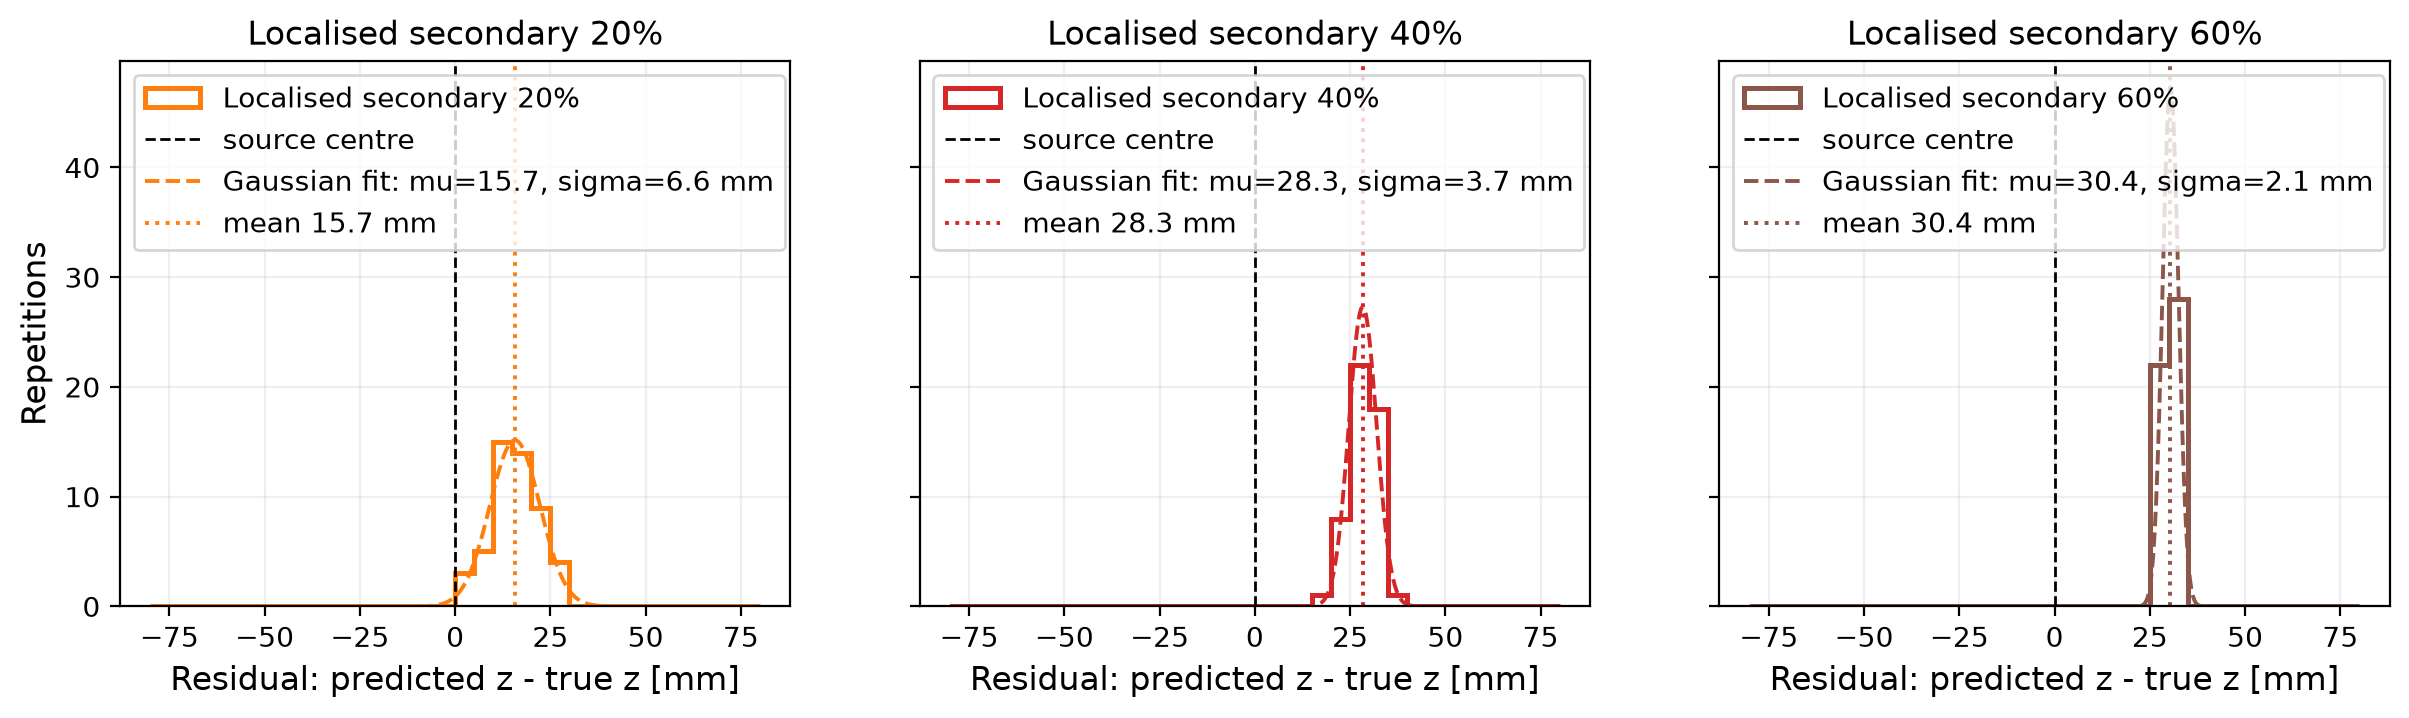
\includegraphics[width=0.98\linewidth]{poster_04b_localised_source_position_residuals.png}
\caption{Localisation residuals across 50 repetitions for each
displaced-source fraction. The dashed black line marks the true source centre;
coloured lines indicate the mean and Gaussian fit.}
\label{fig:source_residuals}
\end{figure}


\begin{figure}[!t]
\centering
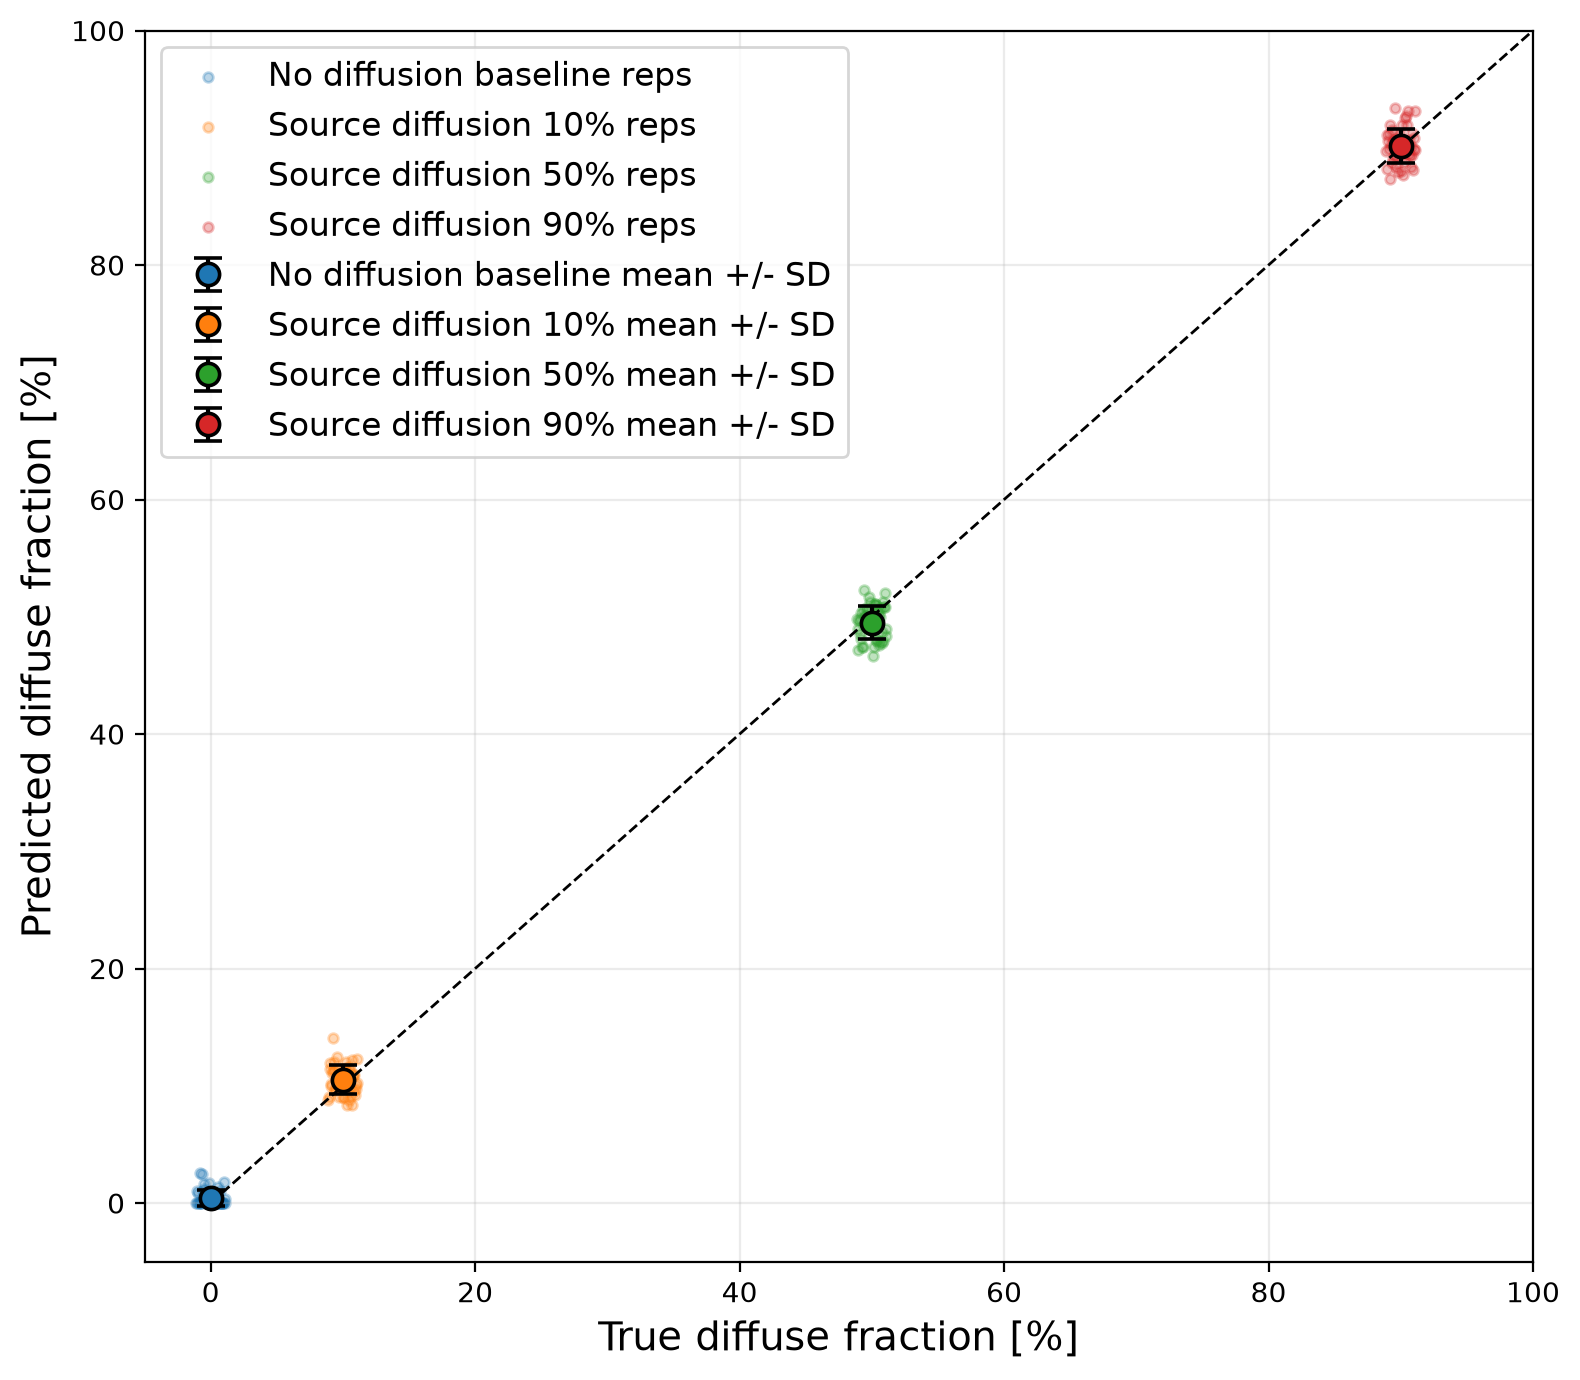
\includegraphics[width=0.72\linewidth]{poster_02_diffusion_fraction_cv_prediction.png}
\caption{Diffusion fraction inferred from 50 independent repetitions. Small
points show individual repetitions and large markers show the mean and
standard deviation.}
\label{fig:diffusion_prediction}
\end{figure}


\begin{figure}[!t]
\centering
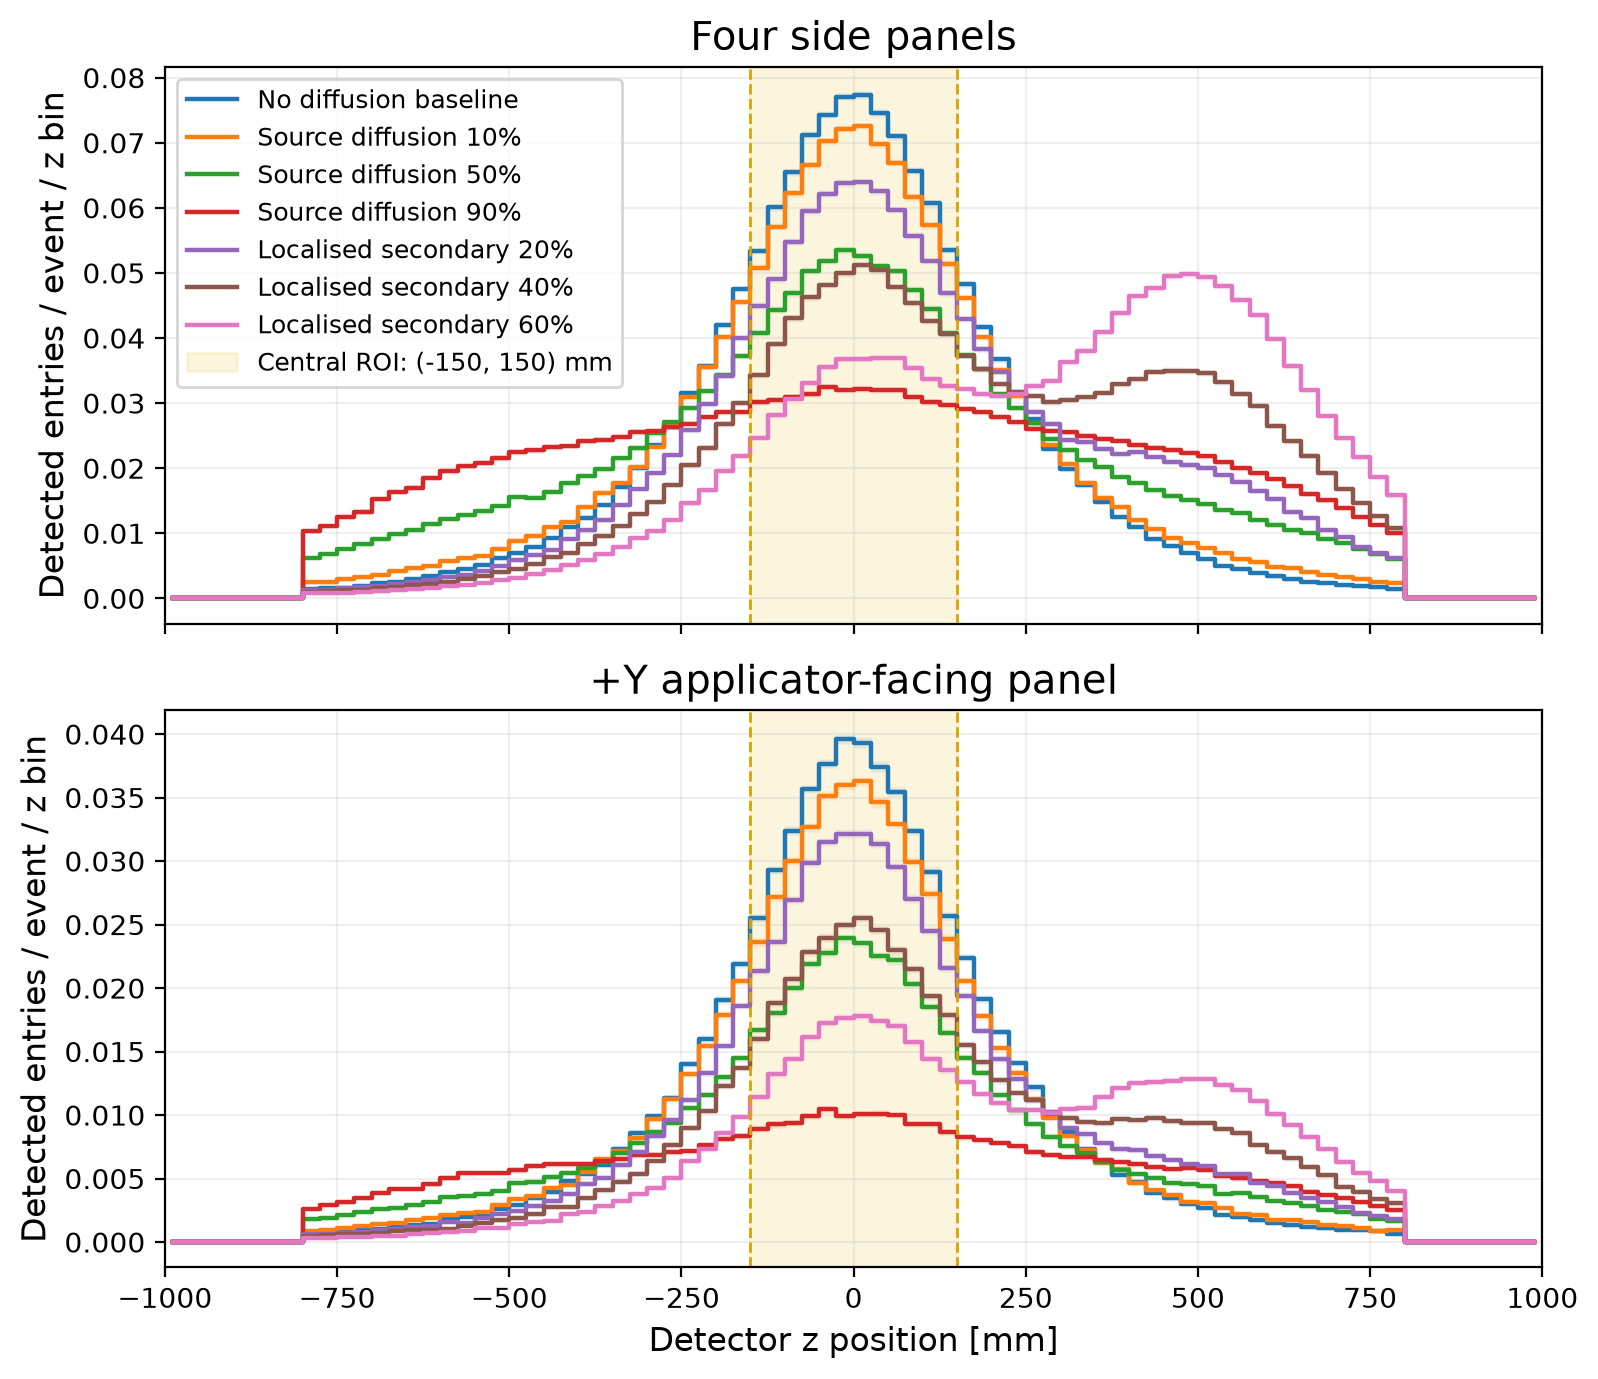
\includegraphics[width=0.65\linewidth]{material_signal_central_roi_profiles.png}
\caption{Central \(|z|\leq150\) mm ROI for the four side panels (top) and the
applicator-facing \(+y\) panel (bottom). The \(+y\) ROI rate provides the
baseline-relative applicator-retained signal.}
\label{fig:central_roi}
\end{figure}
\subsection{Time dependence}
\label{sec:time_results}

Cumulative time-window profiles show that the baseline-subtracted signal is
already visible on hour-scale windows and becomes stronger over longer
observation windows. Across the 50 simulation repetitions, detectability was
defined as a maximum absolute bin-wise residual greater than three times the
combined candidate and baseline standard error. The 50--90\% broad-diffusion and 20--60\%
localised-displacement cases crossed threshold in about 1--2 hours, while the
weaker 10\% broad-diffusion case required about 6 hours. A representative time-window profile is shown in Fig.~\ref{fig:time_windows}. The first threshold-crossing times are summarised in
Table~\ref{tab:time_detection}.

\begin{table}[!t]
\centering
\caption{First \(3\sigma\) detection times from the time-window analysis of
50 independent repetitions.}
\label{tab:time_detection}
\begin{tabular}{lc}
\toprule
Case group & First \(3\sigma\) detection \\
\midrule
10\% broad diffusion & about 6 h \\
50--90\% broad diffusion & about 1--2 h \\
20--60\% localised displacement & about 1--2 h \\
\bottomrule
\end{tabular}
\end{table}

\begin{figure}[!t]
\centering
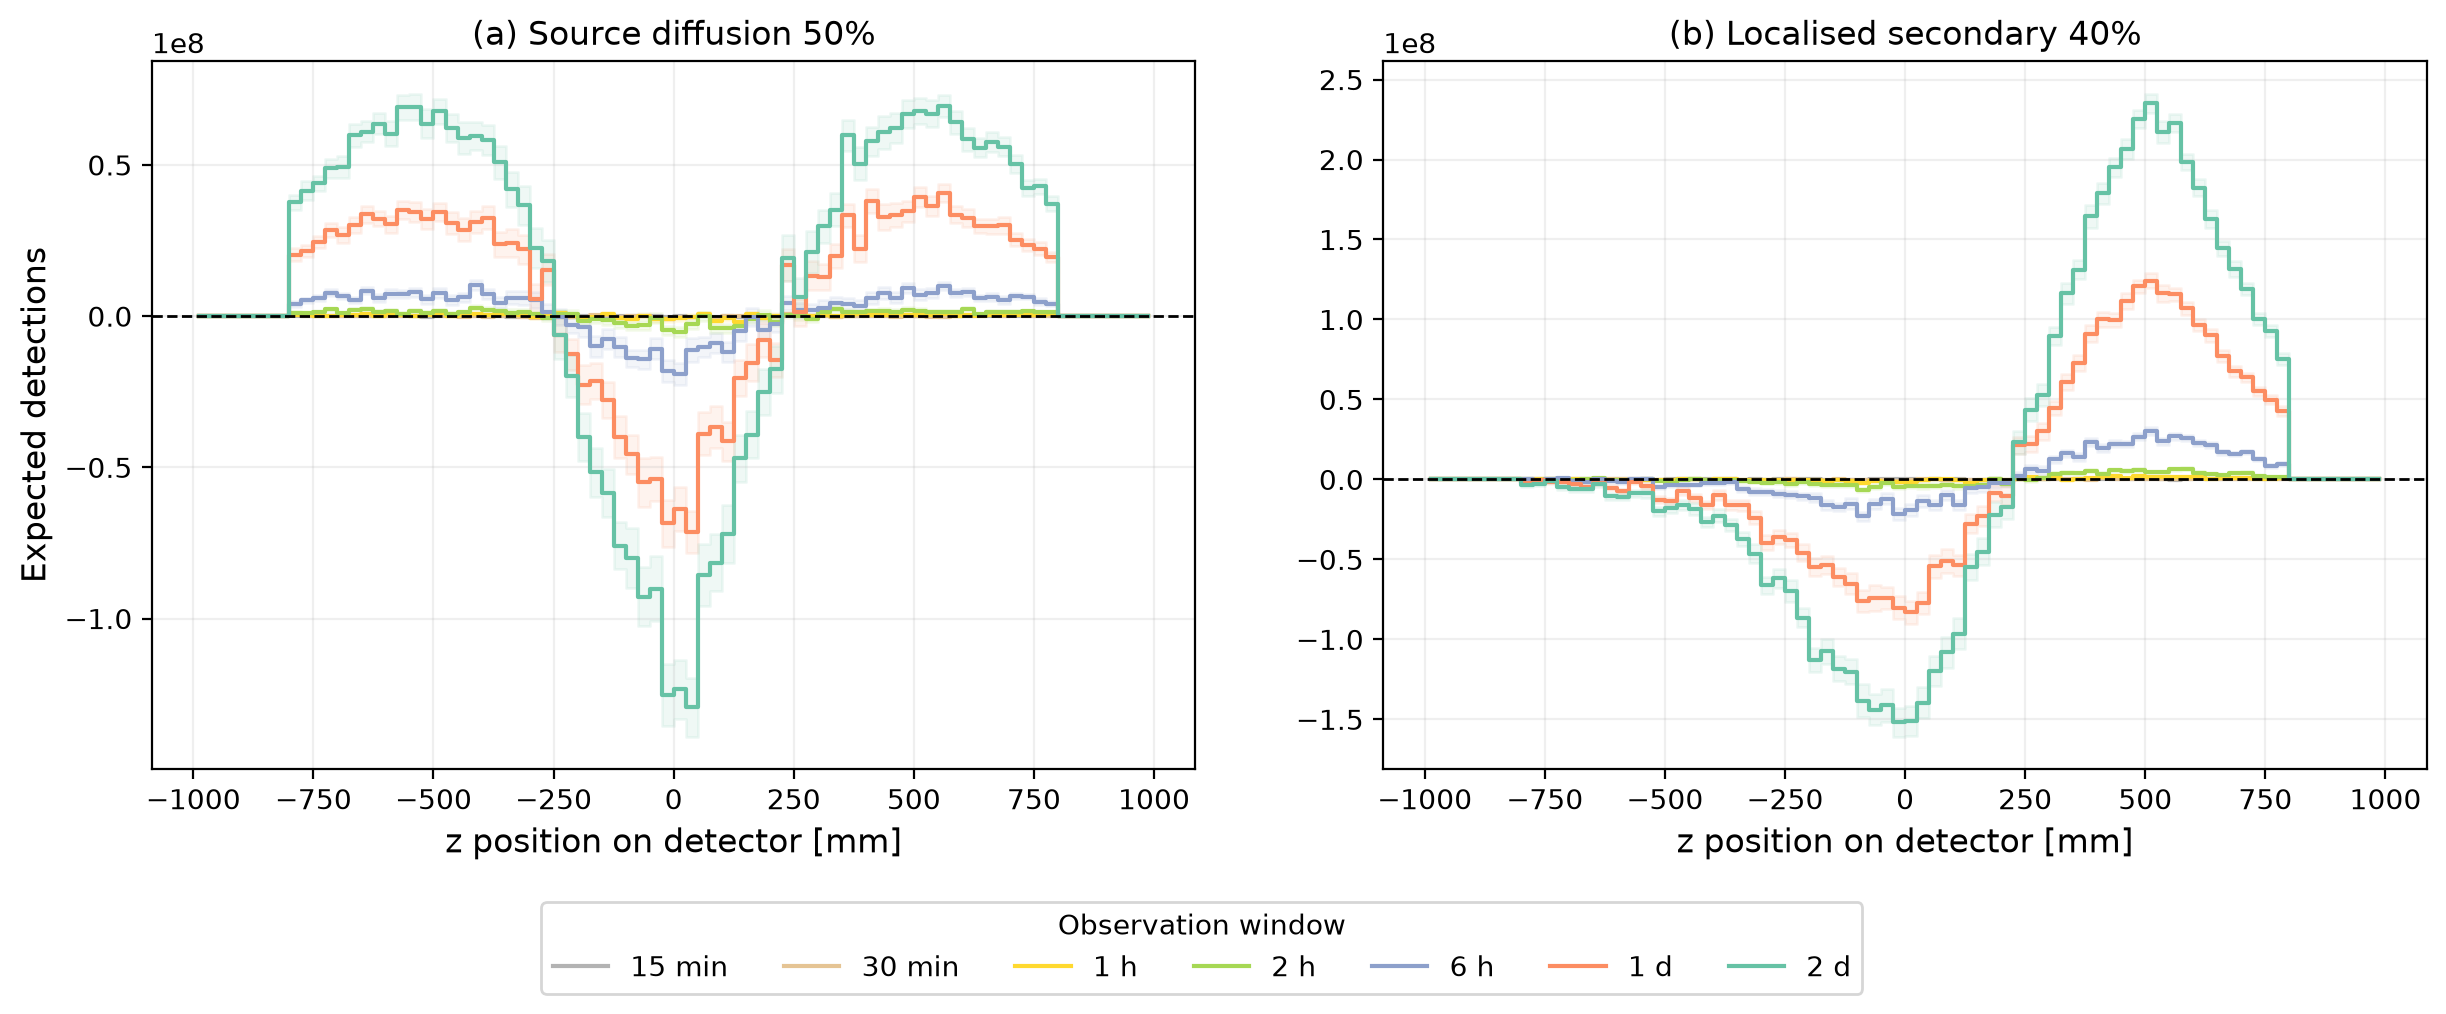
\includegraphics[width=0.82\linewidth]{poster_05_time_window_residual_profiles_diff50_loc40.png}
\caption{Cumulative combined \(+x/-x\) residual profiles for 50\% broad
diffusion (left) and 40\% localised displacement (right). Broad diffusion
produces a symmetric redistribution away from the centre, whereas localised
displacement produces an asymmetric excess near the displaced-source region.
These signatures first exceed the \(3\sigma\) detection threshold after
approximately 2 hours and 1 hour, respectively.}
\label{fig:time_windows}
\end{figure}

\FloatBarrier
\section{Conclusion}

Decay-chain gamma detection provides source-location information and broad redistribution estimation. Baseline-subtracted gamma profiles distinguished retained, broadly redistributed and locally displaced source states. Broad-diffusion fraction was reconstructed with \(R^2=0.9987\) and a mean absolute error of approximately one percentage point. All simulated compact-source cases were detected, with mean reconstructed positions 16–30 mm from the simulated source centre. Depending on the source state, redistribution became detectable after approximately 1–6 hours. 
Broad diffusion and compact source displacement were treated
as independent source states in the present analysis. A combined case, in
which diffuse redistribution and a compact displaced source occur together,
should be included in the next simulation and inference studies. Further work
will also include detector response, background estimation and patient-scale
geometries so that activity-normalised profiles can be interpreted as
experimentally measurable count rates.

\begin{thebibliography}{99}

\bibitem{AlphaGlue2025}
Abu Sabah L \textit{et al.} 2025 AlphaGlue: A novel conceptual delivery method
for $\alpha$ therapy \textit{BioMedInformatics} \textbf{5} 58

\bibitem{Geant4}
Agostinelli S \textit{et al.} 2003 Geant4---a simulation toolkit
\textit{Nucl. Instrum. Methods Phys. Res. A} \textbf{506} 250--303

\bibitem{Geant4DNA}
Incerti S \textit{et al.} 2010 The Geant4-DNA project
\textit{Int. J. Model. Simul. Sci. Comput.} \textbf{1} 157--178

\bibitem{CellCycleAlpha}
Ballisat L \textit{et al.} 2025 Simulation of cell cycle effects on DNA strand
break induction due to $\alpha$-particles \textit{Phys. Med.} \textbf{129}
104871

\bibitem{At211}
De Sio C \textit{et al.} 2025 Targeted alpha therapies using $^{211}$At: A
Geant4 simulation of dose and DNA damage \textit{Phys. Med.} \textbf{129}
104860

\bibitem{DartDoseDNA}
Ballisat L \textit{et al.} 2024 Dose and DNA damage modelling of diffusing
alpha-emitters radiation therapy using Geant4 \textit{Phys. Med.} \textbf{121}
103367

\bibitem{DartInsilico}
Ballisat L \textit{et al.} 2023 In-silico calculations of DNA damage induced
by $\alpha$-particles in the $^{224}$Ra DaRT decay chain for a better
understanding of the radiobiological effectiveness of this treatment
\textit{Phys. Med.} \textbf{112} 102626

\bibitem{laura}
Ballisat L \textit{et al.} 2025 Geant4 simulation of the enhanced in-vivo
$^{220}$Rn spread in DaRT \textit{Phys. Med.} \textbf{135} 105005

\bibitem{heger}
Heger G \textit{et al.} 2024 First measurements of radon-220 diffusion in mice
tumors \textit{Med. Phys.} \textbf{51} 5045--5058

\bibitem{dart}
Arazi L \textit{et al.} 2010 The treatment of solid tumors by alpha emitters
released from $^{224}$Ra-loaded sources \textit{Phys. Med. Biol.} \textbf{55}
1203

\bibitem{RidgeRegression}
Hoerl A E and Kennard R W 1970 Ridge regression: Biased estimation for
nonorthogonal problems \textit{Technometrics} \textbf{12} 55--67
\end{thebibliography}

\end{document}
